\documentclass[]{article}
\usepackage[T1]{fontenc}
\usepackage{lmodern}
\usepackage{graphicx}
\usepackage{amssymb,amsmath}
\usepackage{ifxetex,ifluatex}
\usepackage{fixltx2e} % provides \textsubscript
% use upquote if available, for straight quotes in verbatim environments
\IfFileExists{upquote.sty}{\usepackage{upquote}}{}
\ifnum 0\ifxetex 1\fi\ifluatex 1\fi=0 % if pdftex
  \usepackage[utf8]{inputenc}
\else % if luatex or xelatex
  \ifxetex
    \usepackage{mathspec}
    \usepackage{xltxtra,xunicode}
  \else
    \usepackage{fontspec}
  \fi
  \defaultfontfeatures{Mapping=tex-text,Scale=MatchLowercase}
  \newcommand{\euro}{€}
\fi
% use microtype if available
\IfFileExists{microtype.sty}{\usepackage{microtype}}{}
\ifxetex
  \usepackage[setpagesize=false, % page size defined by xetex
              unicode=false, % unicode breaks when used with xetex
              xetex]{hyperref}
\else
  \usepackage[unicode=true]{hyperref}
\fi
\hypersetup{breaklinks=true,
            bookmarks=true,
            pdfauthor={Lucas Wojciechowski, Dane Carr, Ariel Weingarten},
            pdftitle={ECE457B: Smartwatch Gesture Recognition},
            colorlinks=true,
            citecolor=blue,
            urlcolor=blue,
            linkcolor=magenta,
            pdfborder={0 0 0}}
\urlstyle{same}  % don't use monospace font for urls
\setlength{\parindent}{0pt}
\setlength{\parskip}{6pt plus 2pt minus 1pt}
\setlength{\emergencystretch}{3em}  % prevent overfull lines
\setcounter{secnumdepth}{0}

\author{}
\date{}

\begin{document}

\section{Test}\label{test}

\section{Abstract}

\section{Problem Statement and Solution Motivation}
Wearable technology, such as smartwatches, are poised to become a ubiquitous consumer product. According to businessinsider.com, smartwatches sales are projected to reach 90 million units by 2018 (http://www.businessinsider.com/global-smartwatch-sales-set-to-explode-2014-3). Many user interface paradigms still need to be rethought for these devices to accommodate their small screens and limited input methods. 

\begin{figure}[ht!]
  \centering
  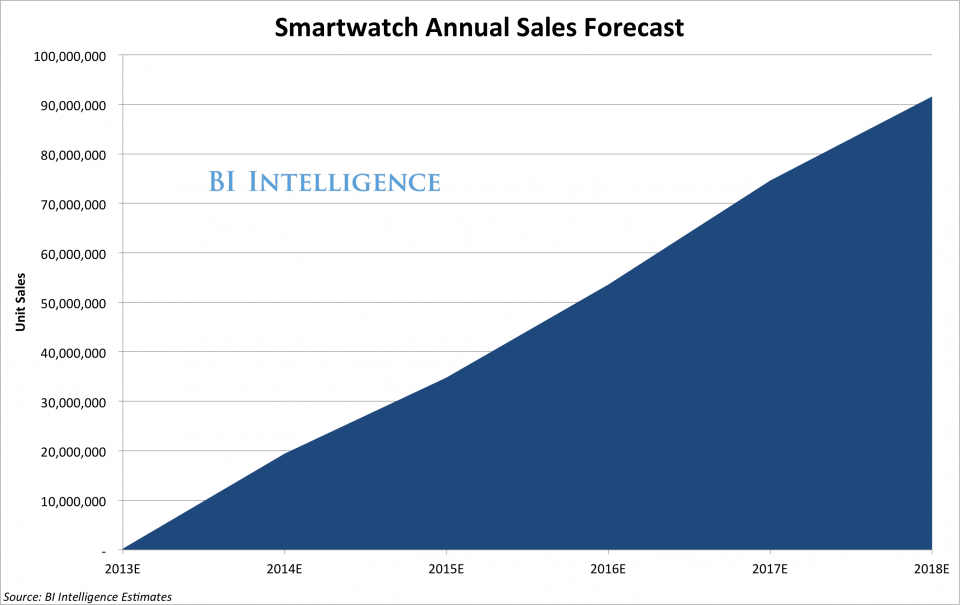
\includegraphics[width=90mm]{smartwatch.png}
  \caption{Smartwatch Annual Sales Projection \label{overflow}}
\end{figure}

Currently, these devices rely mostly on touch input and voice control. Touch input is usually effective, but due to the small form factor, a significant portion of the screen is often obscured by the user's finger. Voice control can be used to complete more complex actions that might be tedious to complete using only touch input, but voice commands are not always practical. They may be less effective in noisy environments, or users might feel uncomfortable using them in public places due to issues with privacy and social acceptance.

Hand and arm gestures could be used to augment existing input paradigms. Though less expressive than voice commands, hand and arm movements are relatively private and they are a natural way to communicate with the environment. There are presently no publicly available gesture recognition solutions for off-the-shelf smartwatches, though theories and interface ideas have been prototyped with other sensors such as Microsoft Kinect or custom ultra-sound detection systems. The potential applications of this technology are far-reaching, from seamless control of Internet-of-things devices to accessibility for visually impaired users.

We have acquired a LG G Watch R and a Nexus 5 phone to record gesture data via a simple, custom-built Android application. Data collected from the watch’s accelerometer will be used to train a neural network to classify a set of simple gestures. We will compare the accuracy and performance of our classifier against similar gesture recognition systems in the research community.

\section{Theoretical Background Material}

\end{document}
